% !TeX spellcheck = ru_RU
% !TEX root = vkr.tex

\section{Обзор}
В этом разделе будут введено и уточнено, что такое деревья квадрантов, техника оптимизации слияние ядер и метапрограмирование на \Th{}.
\subsection{Деревья квадрантов}
Деревья квадрантов~--- рекурсивная структура данных для представления
матриц, чаще всего используется, если матрицы разреженные.
Данная матрица приводится до квадратной с размером, равным степени двойки, далее, если все элементы матрицы равны, то дерево представляется в виде пары значения и размера и  называется листом дерева, в ином случае разделяется на четыре равные части~--- дочерние узлы (квадранты), которые тоже представляют собой деревья квадрантов.
Так происходит пока для каждого родительского узла, не все его дети являются листьями.
Таким образом, строится дерево в привычном для математиков понимания этого слова.
Построенное дерево квадрантов для матрицы

\begin{equation*}
    A =
    \begin{bmatrix}
        1 & 1 &1 & 1\\
        1 & 1 &1 & 1\\
        2 & 2& 4 & 5 \\
        2 & 2 & 6 & 7
    \end{bmatrix}
\end{equation*}
представлено на рис. \ref{qmatrix} и рис. \ref{qtree1}.
Эта структура позволяет \enquote{сжимать} повторяющиеся и находящиеся близко данные в один узел.
\begin{figure}[ht]
    \centering
    % First minipage
    \begin{minipage}[b]{0.45\textwidth}
        \centering
        \resizebox{\linewidth}{!}{
            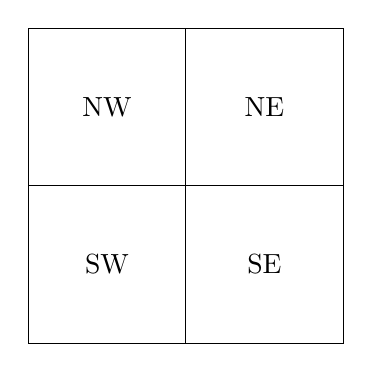
\begin{tikzpicture}
                \draw (1, 1) rectangle (3, 3);
                \draw (1, 3)rectangle (3, 5);
                \draw (3, 1)rectangle (5, 3);
                \draw (3, 3)rectangle (5, 5);
                \node at (2, 2){SW};
                \node at (4, 4){NE};
                \node at (2, 4){NW};
                \node at (4, 2){SE};
            \end{tikzpicture}
        }
        \caption{Квадратная матрица, разделенная на квадранты}
        \label{qmatrix}
    \end{minipage}
    \hfill
    % Second minipage
    \begin{minipage}[b]{0.45\textwidth}
        \centering
        \Tree [.Matrix
                [.NW [] ]
                [.NE [] ]
                [.SW [] ]
                [.SE [] ]
        ]
        \caption{Схематичное изображение одного из узлов дерева квадрантов и его потомков}
        \label{qtree1}
    \end{minipage}
\end{figure}

\newpage
\subsection{Слияние ядер}
Слияние ядер (англ. \textit{kernel fusion}) ~--- техника оптимизации, основанная на идее использования одного блока памяти, необходимого в процессе нескольких вычислений.
В контексте линейной алгебры на деревьях квадрантов ядрами будут служить матрицы, а вычислениями~--- какие-либо функции над ними.

Это работает, потому что для любых операций нужны значения, лежащие в листьях, а для этого необходимо произвести разбор дерева.
Так как матрицы предполагаются одинакового размера (иначе происходит ошибка), если делать это со всеми деревьями одновременно, то можно не только за один проход получить всю необходимую для получения ответа информацию, но ещё и избежать вычисления промежуточных результатов.
\subsection{Метапрограммирование}
Метапрограммирование~--- это процесс создание программ, которые в ходе своего выполнения генерируют другие программы.
В контексте поставленной задачи оно было необходимо, так как
\begin{enumerate}[label=(\alph*)]
    \item нужно генерировать код функций в зависимости от данных, поданных пользователем;
    \item размер этого кода велик, но имеет легко формализуемую структуру.
\end{enumerate}
В \Haskell{} есть встроенная библиотека с обширной и доступной документацией: \Th{}, которая позволяет генерировать код на \Haskell{} во время компиляции.
При этом есть возможность использовать как привычный синтаксис языка, так и более строгие формальные методы для генерации шаблонного кода.
